\documentclass[border=8pt]{standalone}
\usepackage{tikz}
\usetikzlibrary{arrows.meta,positioning,calc,decorations.pathmorphing}
\begin{document}
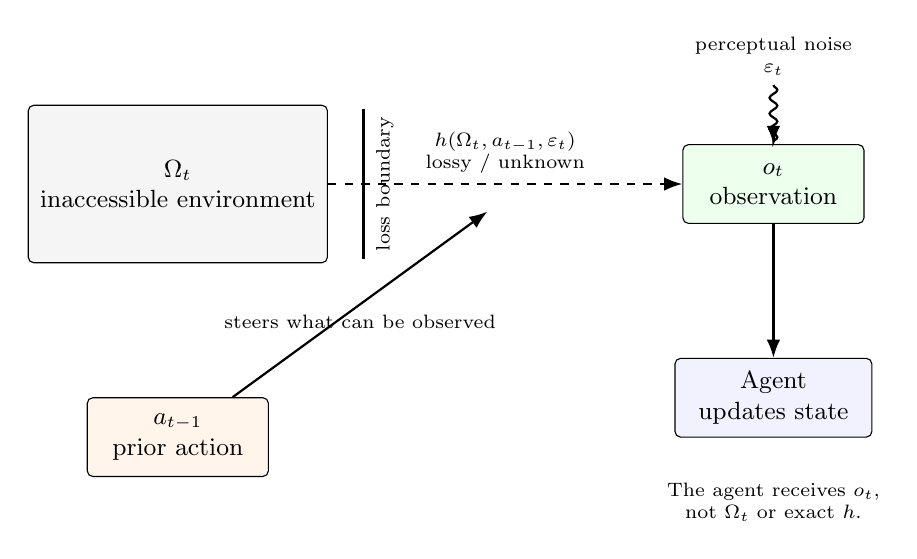
\begin{tikzpicture}[
  world/.style={draw, rounded corners=2pt, align=center, minimum width=3.8cm, minimum height=2.0cm, font=\small, fill=gray!8},
  obs/.style={draw, rounded corners=2pt, align=center, minimum width=2.3cm, minimum height=1.0cm, font=\small, fill=green!7},
  agent/.style={draw, rounded corners=2pt, align=center, minimum width=2.5cm, minimum height=1.0cm, font=\small, fill=blue!5},
  arr/.style={-Latex, thick},
  lossy/.style={-Latex, thick, dashed},
  noise/.style={-Latex, thick, decorate, decoration={snake, amplitude=0.5mm, segment length=2mm}},
  note/.style={align=center, font=\scriptsize}
]

\node[world] (omega) {$\Omega_t$\\inaccessible environment};
\node[obs, right=4.5cm of omega] (o) {$o_t$\\observation};
\node[agent, below=1.7cm of o] (agent) {Agent\\updates state};
\node[obs, below=1.7cm of omega, fill=orange!8] (a) {$a_{t-1}$\\prior action};
\node[note, above=0.75cm of o] (eps) {perceptual noise\\$\varepsilon_t$};

\draw[lossy] (omega) -- node[above, note] {$h(\Omega_t,a_{t-1},\varepsilon_t)$\\lossy / unknown} (o);
\draw[arr] (o) -- (agent);
\draw[arr] (a) -- node[below, note] {steers what can be observed} ($(omega.east)!0.45!(o.west)+(0,-0.35)$);
\draw[noise] (eps) -- (o);

\draw[thick] ($(omega.east)+(0.45,0.95)$) -- ($(omega.east)+(0.45,-0.95)$);
\node[note, rotate=90] at ($(omega.east)+(0.72,0)$) {loss boundary};

\node[note, below=0.45cm of agent] {The agent receives $o_t$,\\not $\Omega_t$ or exact $h$.};

\end{tikzpicture}
\end{document}
